\chapter{ Modelo Lógico}
\par O modelo lógico de uma base de dados representa a fase de transição entre a abstração do modelo conceptual e a implementação técnica no Sistema de Gestão de Base de Dados (SGBD). Nesta etapa, os conceitos e ideias definidos anteriormente são convertidos num modelo representacional, onde as entidades dão lugar a tabelas e os atributos tornam-se colunas com tipos de dados específicos.
\par Ao contrário do modelo conceptual, o modelo lógico foca-se na eficiência da estrutura de dados e nas relações formais. Através de processos de normalização, procura-se obter um conjunto de tabelas que minimizem a redundância e assegurem a integridade referencial, permitindo um registo de dados robusto e coerente com a lógica do mundo real. \\

\begin{figure}[h]
    \centering
    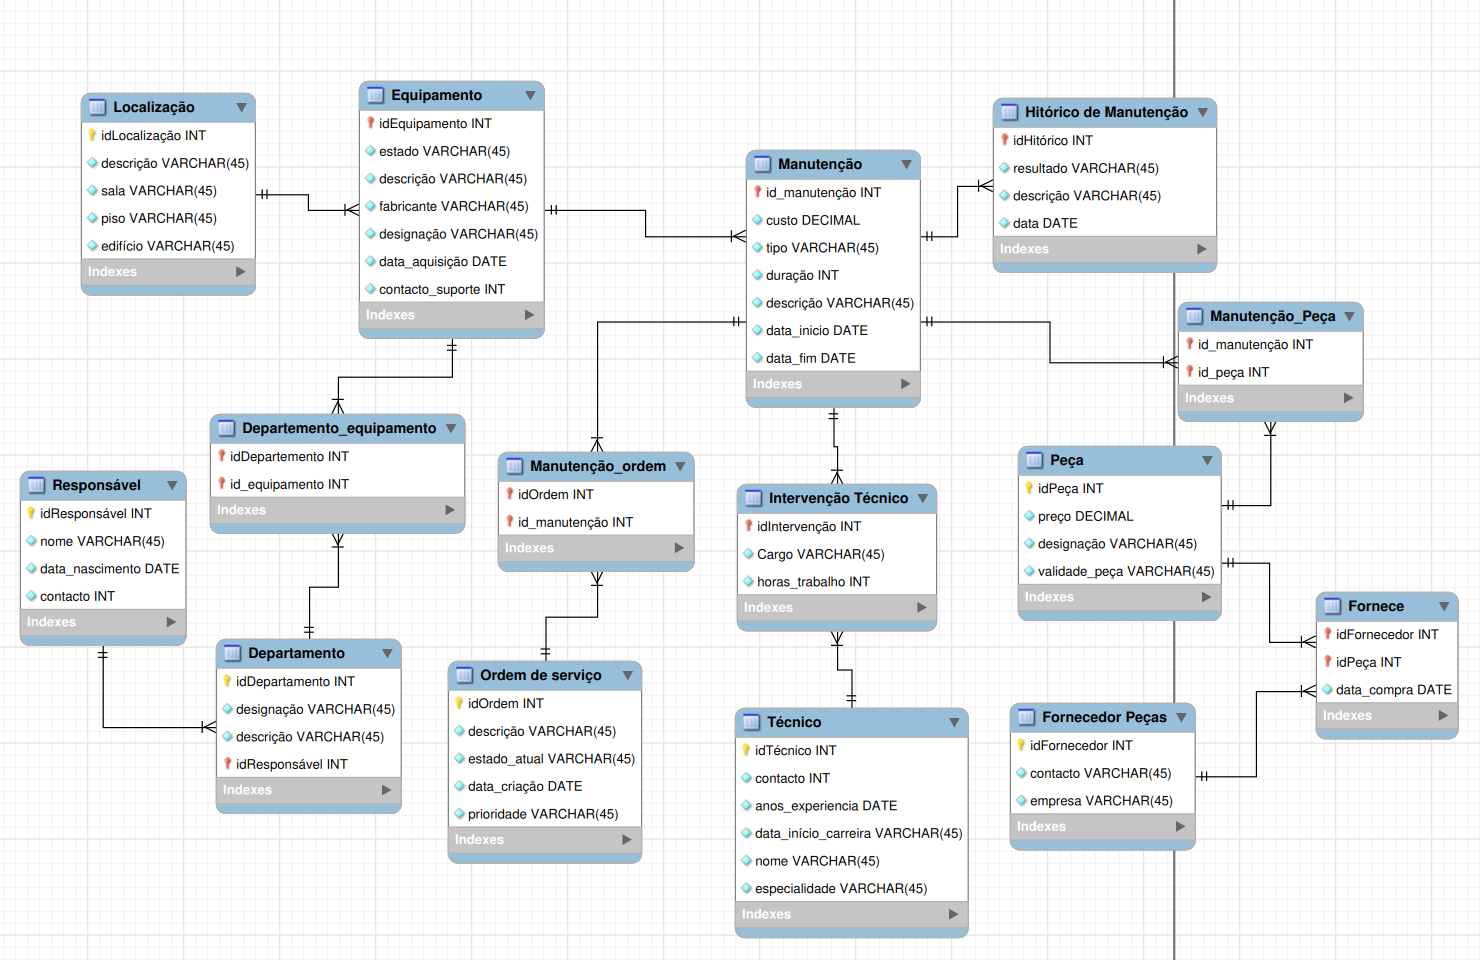
\includegraphics[width=1.05\textwidth]{./03-figuras/modelo_logico}
    \caption{Modelo lógico.}
\end{figure}